% !TEX root =  master.tex
\chapter{Grundlagen}
In diesem Kapitel werden die theoretischen Grundlagen und Gedanken für die Umsetzung im nächsten Kapitel \ref{chap:Implementation} vorgestellt. Die Lösung und das Vorgehen basieren maßgeblich auf dem Beitrag \afz{\MaxLink{https://www.youtube.com/watch?v=YI1WqYKHi78}{Why is this Puzzle Impossible? - Numberphile}} von Herrn Steven Bradlow zur Lösbarkeit des \afz{14-15 puzzles} aus der Einleitung auf dem Youtube Kanal \afz{Numberphile} \autocite{Unsolvable-14-15-Numberphile-YT:online}.%
%
\section{Puzzle zu Listen wandeln} % (fold)
\label{sec:PuzzleToList}
Der Lösungsansatz aus \autocite{Unsolvable-14-15-Numberphile-YT:online} basiert auf Permutationen. Um 4x4 Puzzle besser auf Permutationen untersuchen zu können, werden die Puzzle als Listen von Zahlen dargestellt. Dazu werden die Inhalte der Zellen des Puzzle zeilenweise hintereinander in eine Liste geschrieben. Die Leerstelle, auch als \afz{blank} beschrieben, wird dabei als Zahl \afz{0} interpretiert.
Der Zustand des Puzzle aus Abb.\ref{fig:Perm_puzzle_start_Pic}
\begin{figure}[H]
	\centering
	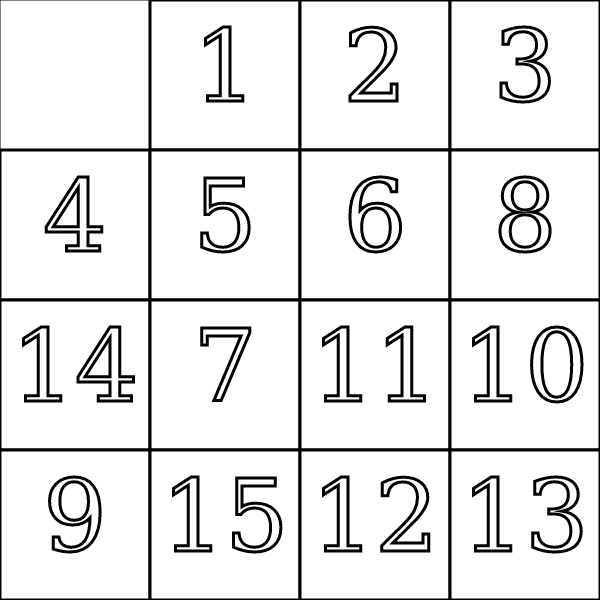
\includegraphics[width=.5\textwidth,keepaspectratio]{img/Start_Puzzle2.png}
	\captionsetup{format=hang}
	\caption{Beispiel Zustand eines 4x4-Puzzle \label{fig:Perm_puzzle_start_Pic}}
\end{figure}
\begin{minipage}{\linewidth}
	wird als Liste aus Zahlen wie folgt dargestellt:
	\begin{center}
		$State = \{0,1,2,3,4,5,6,8,14,7,11,10,9,15,12,13\}$
	\end{center}
\end{minipage}\WNL%
Wichtig ist bei der Betrachtung der lösbaren Puzzle und des Vorgehens der Lösung aus \autocite{Unsolvable-14-15-Numberphile-YT:online} aber auch anderer verfügbarer Quellen \autocite{solving-15-puzzle-lvi:article,geeksforgeeks:online,archer-15-puzzle:article}, dass die Bezeichnung der Leerstelle oder die Art der Konvertierung eines Puzzle zu einer Liste variiert. Die meisten Lösungen sehen den Zielzustand aus Abb.\ref{fig:Perm_puzzle_end_allOther} vor, wobei die Leerstelle dann die Nummer \afz{16} trägt. Um mit den Darstellungen von Herrn Stroetmann aus dem Vorlesungsskript \autocite{github-stroetmann:online} übereinzustimmen, wird der Zielzustand aus Abb.\ref{fig:Perm_puzzle_end_stroet} angestrebt, bei dem die Leerstelle die Nummer \afz{0} trägt.\\
%
\begin{minipage}{\linewidth}
	\begin{minipage}[t]{0.45\linewidth}
		\begin{figure}[H]
			\centering
			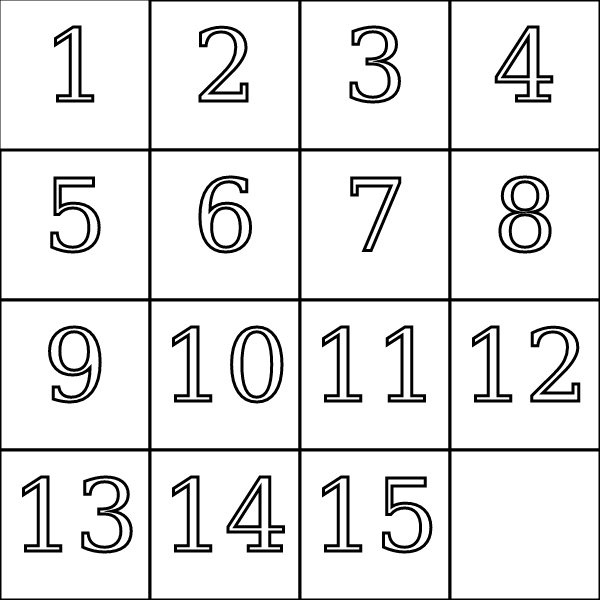
\includegraphics[width=\linewidth,keepaspectratio]{img/End_Puzzle_AO.png}
			\captionsetup{format=plain, indention=0pt}
			\caption{Häufig verwendeter Zielzustand eines 4x4-Puzzle \label{fig:Perm_puzzle_end_allOther}}
		\end{figure}
	\end{minipage}
	\hfill
	\begin{minipage}[t]{0.45\linewidth}
		\begin{figure}[H]
			\centering
			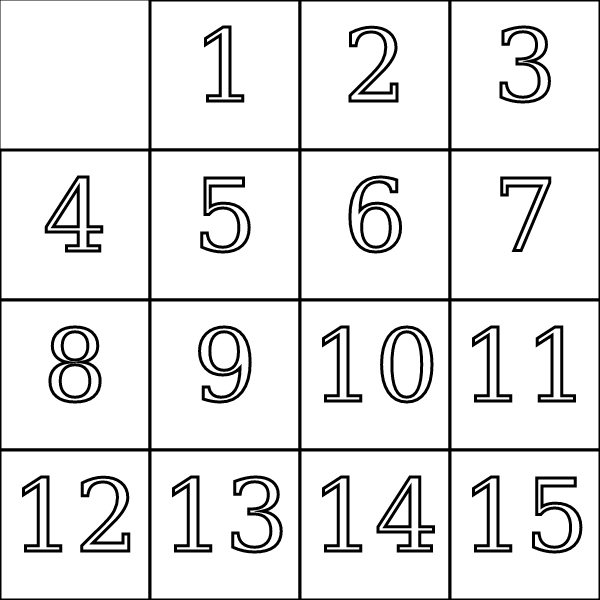
\includegraphics[width=\linewidth,keepaspectratio]{img/End_Puzzle_Stroetmann.png}
			\captionsetup{format=plain, indention=0pt}
			\caption{\label{fig:Perm_puzzle_end_stroet}Verwendeter Zielzustand eines 4x4-Puzzles aus dem Skript von Herrn Stroetmann \autocite{github-stroetmann:online}}
		\end{figure}
	\end{minipage}
\end{minipage}\WNL%

\section{Zustände als Permutationen} % (fold)
\label{sec:Permutation}
Die Grund-Idee der Lösbarkeitsüberprüfung von Bradlow basiert auf dem Vergleichen der Paritäten zwischen benötigten Transpositionen und benötigter Züge zum Verrücken der Leerstelle. Im Folgenden wird die Idee aus seinem Beitrag \autocite{Unsolvable-14-15-Numberphile-YT:online} zusammengefasst vorgestellt.\WNL

Die Vorstellung des Verfahrens beginnt Bradlow damit die Puzzle wie in der vorherigen Sektion in Zahlen Reihen zu wandeln. Durch das Vertauschen von 2 beliebigen Zahlen aus dieser Zahlenreihe entsteht eine Permutation der vorherigen Reihe. Auf diese Weise sei jeder möglicher Zustand in dem sich das Puzzle befinden kann als eine Permutation einer zugrundeliegenden aufsteigend sortieren Zahlenreihe zu sehen. Für diese Permutationen beschreit er die folgenden zwei Eigenschaften:
\begin{enumerate}
	\item[\textbf{E1}] Jede dieser Permutationen lässt sich nur durch das Nutzen von Transpositionen, also dem Vertauschen von Zwei Elementen aus der Liste, während die restlichen gleich bleiben, in eine andere Permutation überführen \cite[Vgl.][7min,07sec]{Unsolvable-14-15-Numberphile-YT:online}.
	\item[\textbf{E2}] Die Anzahl der Schritte, die für das Überführen einer Permutation in eine andere Permutation mithilfe von Transpositionen benötigt wird, ist nicht Festgelegt, aber die Parität dieser Zahl ist fest \cite[Vgl.][10min,13sec]{Unsolvable-14-15-Numberphile-YT:online}.
\end{enumerate}
Basierend auf diesen Eigenschaften fährt er fort, dass die Parität der Anzahl notwendiger Transpositionen durch das zielgerichtete Tauschen der Zahlen, mit dem ziel einer aufsteigen sortieren Zahlenreihe, ermittelt werden kann. Wie in der vorherigen Sektion beschrieben, sieht auch Bradlow die sortierte Zahlenreihe
\begin{center}
	$Goal_{Bradlow} = {1,2,3,4,5,6,7,8,9,10,11,12,13,14,15,16}$
\end{center}
als Abbild des Zielzustandes vor. Daher ist in seinem Vortrag das Ziel der Transpositionen die aufsteigend sortierte Liste. Durch E1 ist sicher gestellt, dass die sortiere Liste erreicht werden kann. E2 begründet, dass die Parität der für die Sortierung notwendigen Transpositionen mit der Parität der notwendigen Züge, wenn das Puzzle lösbar ist, übereinstimmt, obwohl die Regeln des Puzzles nicht betrachtet und somit möglicherweise nicht eingehalten werden.\WNL
Im zweiten Schritt der Lösbarkeitsüberprüfung ermittelt Bradlow die Parität der notwendigen legalen Züge zum Überführen der Leerstelle aus dem Startzustand zum Zielzustand. Dabei ist ebenfalls jeder einzelne Zug als eine Transposition zu sehen.\WNL%
Lösbar ist ein Puzzle nach Bradlow dann, wenn die ermittelten Paritäten übereinstimmen. Denn nach E2 sind die Paritäten festgelegt und können nicht verändert werden. Die Parität der Leerstellen Bewegung ist Legal, während Parität der notwendigen zur Sortierung notwendigen Züge nur hypothetisch sind. stimmen die Paritäten nicht über ein existiert nach E2 keine Möglichkeit beide Ziele, also die Sortierung ebenso wie das einhalten Zugregeln einzuhalten. 
\WNL
In der nächsten Sektion wird dieses Verfahren an einem Beispiel schrittweise durchgegangen.
\WNL
Für die Sektion \ref*{cha:Umsetzung}, soll noch erwähnt werden, dass sich die Leerstelle nur horizontal und vertikal \afz{bewegen} darf und sich die Anzahl der Züge so mithilfe der Manhattan-Distanz ermitteln lässt.


\section{Kontext Vorlesung + Abgrenzung} % (fold)
\label{cha:Kontext Vorlesung}

% chapter Kontext Vorlesung (end)
\section{Sortieralgorithmen} % (fold)
\label{cha:Sortieralgorithmen}
Mit Ordnung?!
% chapter Sortieralgorithmen (end)
% Endzustände sind nicht ineinander überführbar
% Betrachtung von 2x2 Puzzle um zu zeigen dass es immer 2pfade gibt
% Betrachtung des Loyd Puzzles
% Betrachtung der einen Vorgegebenen Lösung von Herrn Stroetmann 

